\chapter{Comparaison entre Gadget et un code Vlasov\label{Chap::VlasovGadget}}
	\minitoc%

	\todo[inline]{Ce chapitre en est à peine à son premier jet. Toutes les figures ne sont pas encore commenté (ça arrivera dans le courant de la
	semaine). Il manque aussi les figures contenant tous les $j$ sommé.}

	% Une des questions qui se posent avec notre approche concerne sa validité. En effet, à quel point gadget peut il
	% être proche d'un programme résolvant directement les équations de Vlasov-Poisson. Dans ce chapitre, nous tentons
	% d'apporter des éléments de réponse.

	Avant de présenter les résultats obtenus au cours de la thèse, nous allons présenter un travail que nous avons effectué en parallèle. Il a été
	effectué conjointement avec Stéphane Colombi, Thierry Sousbie et Sébastien Peirani. Il consiste à comparer les résultats donnés par un code
	résolvant numériquement l'équation de Vlasov (écrit par Thierry Sousbie en se basant sur~\cite{1983PASJ...35..547F}) et le code $N$-corps
	\textsc{gadget-2}.

	Tous les diagrammes de l'espace des phases, sauf si précisé, présente à gauche la simulation Vlasov et à droite la simulation
	\textsc{gadget-2}. Tous sont normalisés de façon à utiliser la même échelle de couleurs pour une même simulation.

	\section{Description du code Vlasov}

		Nous considérons un système à symétrie sphérique. L'équation de Vlasov s'écrit:
		\begin{align}
			\pderivn{f}{t} + v_r\pderivn{f}{r} + \(\dfrac{j^2}{r^3} - \dfrac{GM(r)}{r^2}\)\pderivn{f}{v_r} = 0\label{Eq::ValGad::Pois}
		\end{align}
		avec $f = f(r, u, j, t)$ la fonction de distribution dans l'espace des phases du système au temps $t$, $r$ le rayon de l'objet, $v_r$
		la vitesse radiale et $j$ le moment angulaire. La fonction $M(r)$ donne la masse contenue à l'intérieur de la sphère de rayon $r$.

		Pour résoudre l'équation, l'espace des phases $\(r, v_r, j\)$ est discrétisé sur un maillage tridimensionnel de dimension $(r, v_r,
		j)\in\(\left[r_\mathrm{min}; r_\mathrm{max}\right], \left[-v_r^\mathrm{max}; v_r^\mathrm{max}\right], \left[0;
		j_\mathrm{max}\right]\)$ avec $r$ évoluant logarithmiquement. Chaque point du maillage est considéré comme une particule.
		L'équation~\refeq{Eq::ValGad::Pois} est séparée en deux opérateurs:
		\begin{itemize}
			\item un premier opérateur permet d'obtenir la trajectoire d'une particule libre:
				\begin{align*}
					\pderivn{f}{t} + v_r\pderivn{f}{r} + \dfrac{j^2}{r^3}\pderivn{f}{u} = 0
				\end{align*}
			\item un second permettant de calculer l'accélération:
				\begin{align*}
					\pderivn{f}{t} - \dfrac{GM(r)}{r^2}\pderivn{f}{v_r} = 0
				\end{align*}
		\end{itemize}
		Ces deux opérateurs, alliés à un schéma de type \og\sm\fg, % \og{}Leap-frog\fg,
		vont permettre de faire évoluer la position chaque
		point du maillage du temps $t$ au temps $t+dt$. Puis, profitant du fait que toutes les couche de moment angulaire est indépendante des
		autres, une interpolation de la fonction de distribution dans le plan $\(r, v_r\)$ pour chaque $j$ permet de reconstruire le maillage.

		L'axe selon $r$ évoluant logarithmiquement, un problème va se poser lorsque $r\to0$. Pour l'éviter, nous faisons l'approximation que
		les particules à l'intérieur du rayon $r_\mathrm{min}$ sont libres. Ce rayon doit donc être suffisamment petit pour que cette approximation
		soit vérifié, mais suffisamment grand pour éviter la divergence du logarithme.
		% toutes les particules passant sous ce rayon $r_\mathrm{min}$ puissent évoluer comme des particules libres.

		Plus de détails sur le fonctionnement du code pourront être trouvés dans l'article associé à cette étude (référence?). Pour effectuer
		la comparaison de ce code à \textsc{gadget-2}, nous allons utiliser une sphère de Hénon de viriel $\gamma$. À cause de certaines limitations
		inhérentes à l'interpolation, nous avons dû lisser cette sphère en multipliant la fonction de distribution par la fonction:
		\begin{align*}
			g(r) = \mathrm{erf}\( \dfrac{R - r }{ r_\epsilon }\) + 1
		\end{align*}
		avec $R$ est le rayon de l'objet et $r_\epsilon$ le rayon sur lequel la sphère sera lissée.

		Dans les sections suivantes, nous allons comparer ces deux codes en utilisant deux rapports du viriel: $\gamma=-0,5$ et $\gamma=-0,1$.
		% l'évolution de la sphère de Hénon avec un viriel de $\gamma=-0,5$ puis nous
		% enchaînerons sur une comparaison utilisant un viriel de $\gamma=-0.1$.

	\section{Comparaison pour $\gamma = -0,5$}

		Nous allons commencer par comparer nos deux codes numériques dans le cadre de conditions initiales dont l'évolution est bien connue et
		décrite dans la littérature: nous allons regarder/étudier l'effondrement d'une sphère de Hénon de viriel $\gamma=-0,5$. Nous prenons comme
		référence l'article de~\cite{1983PASJ...35..547F}. Nous nous placerons dans le même système d'unités.

		Pour comparer nos simulations, nous nous baserons sur la correspondance entre l'espace des phases $(r, v_r)$ pour $j=0,425$, l'espace
		des phases intégré sur $j$ et l'évolution du profil de densité de l'objet. Nous effectuerons ces comparaison à différents temps afin
		de montrer que nous obtenons bien le même comportement au cours du temps. La simulation \textsc{gadget-2} utilisée ici comporte $10^6$
		particules. L'article associé étudiera aussi l'évolution de simulations composées de $10^5$ et $10^7$ particules.

		\todo[inline]{L'impact du lissage de la force. À rédiger selon ce qui est dit dans l'article. Pas possible de présenter l'étude sur le
		pas de temps, je n'ai rien d'utilisable.}

		\subsection{Effet du lissage de la force}

			Un paramètre important de la simulation va être le paramètre de lissage de la force $\epsilon$. Ce paramètre va influencer sur
			la dynamique en donnant ou retirant de l'importance au collision. Nous avons donc effectué des simulations d'une sphère de
			Hénon lissée, de viriel $\gamma=-0,5$, avec différents $\epsilon$. La figure~\ref{Fig::ValGad::0.5::SoftAll} montre l'espace
			des phases pour chaque $\epsilon$ utilisé.
			\begin{figure}[htbp]
				\begin{subfigure}{0.5\linewidth}
					\centering 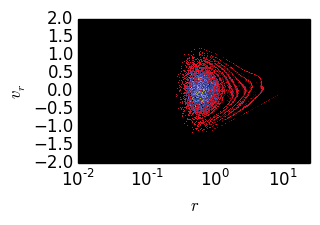
\includegraphics{{vlasov_gadget/Vlasov_0.5_Soft/CompVlasGad_512_0.5_0.0001}.png}
					\centering \caption{$\epsilon=10^{-4}$\label{Fig::ValGad::0.5::Soft1}}
				\end{subfigure}\hfill
				\begin{subfigure}{0.5\linewidth}
					\centering 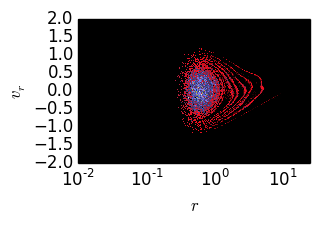
\includegraphics{{vlasov_gadget/Vlasov_0.5_Soft/CompVlasGad_512_0.5_0.001}.png}
					\centering \caption{$\epsilon=10^{-3}$\label{Fig::ValGad::0.5::Soft2}}
				\end{subfigure}
				\begin{subfigure}{0.5\linewidth}
					\centering 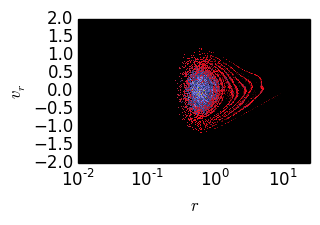
\includegraphics{{vlasov_gadget/Vlasov_0.5_Soft/CompVlasGad_512_0.5_0.01}.png}
					\centering \caption{$\epsilon=10^{-2}$\label{Fig::ValGad::0.5::Soft3}}
				\end{subfigure}\hfill
				\begin{subfigure}{0.5\linewidth}
					\centering 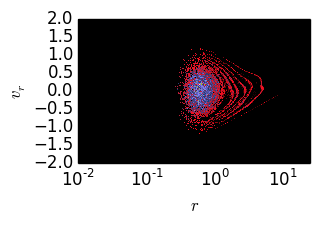
\includegraphics{{vlasov_gadget/Vlasov_0.5_Soft/CompVlasGad_512_0.5_0.1}.png}
					\centering \caption{$\epsilon=10^{-1}$\label{Fig::ValGad::0.5::Soft4}}
				\end{subfigure}
				\caption{Représentation de l'espace des phase à $j=0.425$ et $t=45$ pour $\gamma=-0,5$ et différents
					$\epsilon$.\label{Fig::ValGad::0.5::SoftAll}}
			\end{figure}
			Nous pouvons voir sur ces figures que l'espace des phases est très similaires, et ne semble pas dépendre de la valeur de
			$\epsilon$. Les enroulements à grand $r$ montrent les mêmes variations entre chaque diagrammes.

		\subsection{Comparaison entre les simulations Vlasov et \textsc{Gadget-2}}

			Après avoir montré que le lissage de la force n'avait pas d'influence sur l'évolution du Hénon, nous allons comparer nos
			simulations \textsc{gadget-2} avec les simulations Vlasov en utilisant $\epsilon=10^{-3}$. La première chose que nous
			vérifions est la conservation de la sphéricité de la sphère.
			\begin{figure}[htbp]
				\begin{minipage}{0.45\linewidth}
					\begin{center}
					\centering 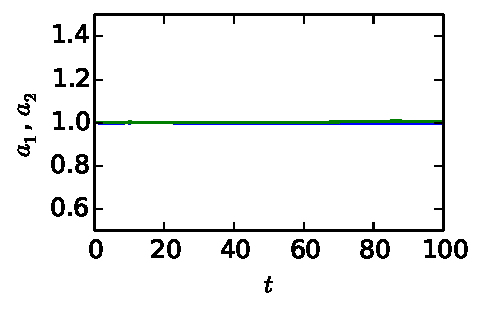
\includegraphics{{vlasov_gadget/AxialRatio_0.5}.pdf}
					\centering \caption{Évolution des rapports d'axes $a_1$ et $a_2$ pour $\gamma=-0,5$.\label{Fig::VlaGad::SpheTest::AR}}
					\end{center}
				\end{minipage}
				\begin{minipage}{0.45\linewidth}
					\begin{center}
					\centering 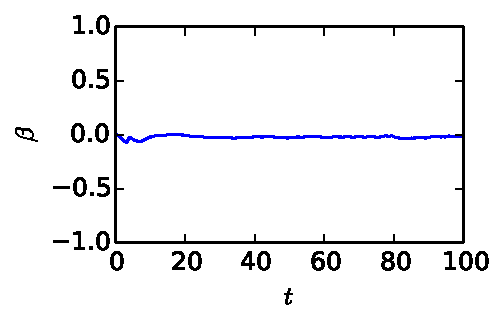
\includegraphics{{vlasov_gadget/Anisotropy_0.5}.pdf}
					\centering \caption{Évolution de l'anisotropie pour $\gamma=-0,5$.\label{Fig::VlaGad::SpheTest::Aniso}}
					\end{center}
				\end{minipage}
			\end{figure}
			C'est ce que montre la figure~\ref{Fig::VlaGad::SpheTest::AR}
			représentant l'évolution des rapports d'axes au cours du temps. Ils restent tous deux très proches de $1$. La sphère de Hénon
			reste bien sphérique tout du long de son évolution. La figure~\ref{Fig::VlaGad::SpheTest::Aniso} montre l'évolution de
			l'anisotropie au cours. Son évolution confire que la sphère conserve son anisotropie tout au long de son évolution.

			Le premier temps que nous regardons est $t=0$. La figure~\ref{Fig::ValGad::0.5::t0} montre l'espace des phases pour les conditions
			initiales. La première chose à noter concerne la différence apparente concernant le maximum de la fonction de distributions. Cette
			différence est dû au faible nombre de particules présentes dans la couche de $j$ choisi. Excepté ce point, nous retrouvons bien la
			croissance progressive du nombre de particule ainsi qu'un étalement progressif des vitesses radiales quand $r$ augmente.
			\begin{figure}[htbp]
				\begin{minipage}{1.00\linewidth}
					\centering \includegraphics[width=\linewidth]{{CompVlasGad_t_0_512_0.5}.png}
					\caption{Comparaison de l'espace des phases entre le code vlasov (à gauche) et le code Gadget (à droite), à $t=0$ et pour $j=0,425$.\label{Fig::ValGad::0.5::t0}}
				\end{minipage}\hfill
				\begin{minipage}{1.00\linewidth}
					\centering \includegraphics{{CompVlasGad_Density_0.5_t_0_error}.pdf}
					\caption{Comparaison du profil de densité entre le code vlasov (en bleu) et le code gadget (en vert), pour $t=0$.\label{Fig::ValGad::0.5::Density::t0}}
				\end{minipage}
			\end{figure}
			Du côté du profil de densité (figure~\ref{Fig::ValGad::0.5::Density::t0}), l'accord est très bon, excepté au centre du système où le manque de particules empêche le calcul précis
			de la densité.

			Le deuxième temps que nous avons choisi de montrer se situe peu après la fin de l'effondrement de la sphère de Hénon. Le nombre
			d'enroulement présent sur les graphiques de la figure~\ref{Fig::ValGad::0.5::t13} sont les mêmes. Par contre, l'enroulement central
			donne de la simulation gadget semble un peu en avance sur la simulation vlasov. Ce qui semble confirmé par le \og{}bras\fg s'étendant
			jusqu'à $r=3$ pour la simulation vlasov et jusqu'à $r=4$ pour la simulation gadget.
			\begin{figure}[htbp]
				\begin{minipage}{1.00\linewidth}
					\centering \includegraphics[width=\linewidth]{{CompVlasGad_t_13_512_0.5}.png}
					\caption{Comparaison de l'espace des phases entre le code vlasov (à gauche) et le code Gadget (à droite), à $t=13$ et pour $j=0,425$.\label{Fig::ValGad::0.5::t13}}
				\end{minipage}\hfill
				\begin{minipage}{1.00\linewidth}
					\centering \includegraphics{{CompVlasGad_Density_0.5_t_13_error}.pdf}
					\caption{Comparaison du profil de densité entre le code vlasov (en bleu) et le code gadget (en vert), pour $t=13$.\label{Fig::ValGad::0.5::Density::t13}}
				\end{minipage}
			\end{figure}
			Les profils de densité présenté sur la figure~\ref{Fig::ValGad::0.5::Density::t13} montre par contre un très bon accord, excepté au
			bord du système, où le nombre de particules recommence alors à faiblir. L'extension du système en $r$ est aussi visible.
			% \begin{figure}[htpb]
			% \end{figure}
			Cette extension du profil peut-être expliqué par l'éjection d'une fraction des particules hors du système suite aux collisions se
			produisant dans le système.

			Pour terminer la comparaison à ce viriel, nous regardons ce qu'il se passe à $t=45$. À ce moment, le système a eu le temps de se
			stabiliser. Nous remarquons, en regardant la figure~\ref{Fig::ValGad::0.5::t45}, que la simulation gadget présente des
			\og{}vaguelettes\fg sur les enroulements extérieurs qui semble en avance sur la simulation vlasov.
			\begin{figure}[htbp]
				\begin{minipage}{1.00\linewidth}
					\centering \includegraphics[width=\linewidth]{{CompVlasGad_t_45_512_0.5}.png}
					\caption{Comparaison de l'espace des phases entre le code vlasov (à gauche) et le code Gadget (à droite), à $t=45$ et pour $j=0,425$.\label{Fig::ValGad::0.5::t45}}
				\end{minipage}\hfill
				\begin{minipage}{1.00\linewidth}
					\centering \includegraphics{{CompVlasGad_Density_0.5_t_45_error}.pdf}
					\caption{Comparaison du profil de densité entre le code vlasov (en bleu) et le code gadget (en vert), pour $t=45$.\label{Fig::ValGad::0.5::Density::t45}}
				\end{minipage}
			\end{figure}


	\section{Comparaison pour $\gamma = -0,1$}

		Comme pour la comparaison précédente, nous allons commencer par vérifier que le système conserve ses propriété de sphéricité et
		d'isotropie.
		\begin{figure}[htbp]
			\begin{minipage}{0.45\linewidth}
				\begin{center}
				\centering 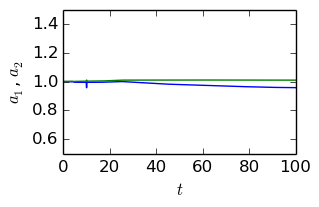
\includegraphics{{vlasov_gadget/AxialRatio_0.1}.pdf}
				\centering \caption{Évolution des rapports d'axes $a_1$ et $a_2$ pour
				$\gamma=-0,1$.\label{Fig::VlaGad::SpheTest::AR0.1}}
				\end{center}
			\end{minipage}
			\begin{minipage}{0.45\linewidth}
				\begin{center}
				\centering 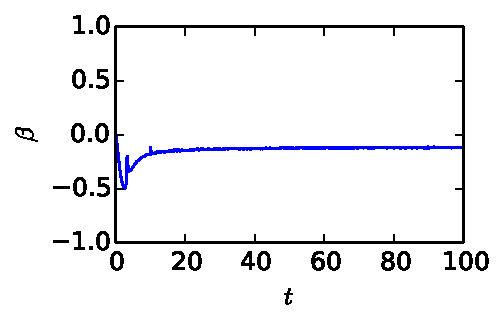
\includegraphics{{vlasov_gadget/Anisotropy_0.1}.pdf}
				\centering \caption{Évolution de l'anisotropie pour $\gamma=-0,1$.\label{Fig::VlaGad::SpheTest::Aniso0.1}}
				\end{center}
			\end{minipage}
		\end{figure}
		C'est ce que montre les figure~\ref{Fig::VlaGad::SpheTest::AR} et~\ref{Fig::VlaGad::SpheTest::Aniso}. Ces deux observables confirment
		donc que l'objet reste bien sphérique et isotrope.

		Le premier temps que nous regardons est $t=0$. La figure~\ref{Fig::ValGad::0.1::t0} montre l'espace des phases pour les conditions
		initiales. La première chose à noter concerne la différence apparente concernant le maximum de la fonction de distributions. Cette
		différence est dû au faible nombre de particules présentes dans la couche de $j$ choisi. Excepté ce point, nous retrouvons bien la
		croissance progressive du nombre de particule ainsi qu'un étalement progressif des vitesses radiales quand $r$ augmente.
		\begin{figure}[htbp]
			\begin{minipage}{1.00\linewidth}
				\centering \includegraphics[width=\linewidth]{{CompVlasGad_t_0_512_0.1}.png}
				\caption{Comparaison de l'espace des phases entre le code vlasov (à gauche) et le code Gadget (à droite), à $t=0$ et pour $j=0,425$.\label{Fig::ValGad::0.1::t0}}
			\end{minipage}\hfill
			\begin{minipage}{1.00\linewidth}
				\centering \includegraphics{{CompVlasGad_Density_0.1_t_0_error}.pdf}
				\caption{Comparaison du profil de densité entre le code vlasov (en bleu) et le code gadget (en vert), pour $t=0$.\label{Fig::ValGad::0.1::Density::t0}}
			\end{minipage}
		\end{figure}
		Du côté du profil de densité (figure~\ref{Fig::ValGad::0.1::Density::t0}), l'accord est très bon, excepté au centre du système où le manque de particules empêche le calcul précis
		de la densité.

		Le deuxième temps que nous avons choisi de montrer se situe peu après la fin de l'effondrement de la sphère de Hénon. Le nombre
		d'enroulement présent sur les graphiques de la figure~\ref{Fig::ValGad::0.1::t13} sont les mêmes. Par contre, l'enroulement central
		donne de la simulation gadget semble un peu en avance sur la simulation vlasov. Ce qui semble confirmé par le \og{}bras\fg s'étendant
		jusqu'à $r=3$ pour la simulation vlasov et jusqu'à $r=4$ pour la simulation gadget.
		\begin{figure}[htbp]
			\begin{minipage}{1.00\linewidth}
				\centering \includegraphics[width=\linewidth]{{CompVlasGad_t_5_512_0.1}.png}
				\caption{Comparaison de l'espace des phases entre le code vlasov (à gauche) et le code Gadget (à droite), à $t=5$ et pour $j=0,425$.\label{Fig::ValGad::0.1::t13}}
			\end{minipage}\hfill
			\begin{minipage}{1.00\linewidth}
				\centering \includegraphics{{CompVlasGad_Density_0.1_t_5_error}.pdf}
				\caption{Comparaison du profil de densité entre le code vlasov (en bleu) et le code gadget (en vert), pour $t=5$.\label{Fig::ValGad::0.1::Density::t13}}
			\end{minipage}
		\end{figure}
		Les profils de densité présenté sur la figure~\ref{Fig::ValGad::0.1::Density::t13} montre par contre un très bon accord, excepté au
		bord du système, où le nombre de particules recommence alors à faiblir. L'extension du système en $r$ est aussi visible.
		% \begin{figure}[htpb]
		% \end{figure}
		Cette extension du profil peut-être expliqué par l'éjection d'une fraction des particules hors du système suite aux collisions se
		produisant dans le système.

		Pour terminer la comparaison à ce viriel, nous regardons ce qu'il se passe à $t=45$. À ce moment, le système a eu le temps de se
		stabiliser. Nous remarquons, en regardant la figure~\ref{Fig::ValGad::0.1::t45}, que la simulation gadget présente des
		\og{}vaguelettes\fg sur les enroulements extérieurs qui semble en avance sur la simulation vlasov.
		\begin{figure}[htbp]
			\begin{minipage}{1.00\linewidth}
				\centering \includegraphics[width=\linewidth]{{CompVlasGad_t_25_512_0.1}.png}
				\caption{Comparaison de l'espace des phases entre le code vlasov (à gauche) et le code Gadget (à droite), à $t=25$ et pour $j=0,425$.\label{Fig::ValGad::0.1::t45}}
			\end{minipage}\hfill
			\begin{minipage}{1.00\linewidth}
				\centering \includegraphics{{CompVlasGad_Density_0.1_t_25_error}.pdf}
				\caption{Comparaison du profil de densité entre le code vlasov (en bleu) et le code gadget (en vert), pour $t=25$.\label{Fig::ValGad::0.1::Density::t45}}
			\end{minipage}
		\end{figure}

